\qrchapter{https://forgottenpillar.com/rsc/pl-fp-chapter23}{Wielkie odstępstwo wkrótce się urzeczywistni} \label{chap:apostasy}

W 1903 roku, gdy opublikowano \textit{The Living Temple} i wywołano spór wokół \emcap{osobowości Boga}, siostra White wiernie wypełniała polecenie Wielkiego Dowódcy. Została wezwana słowami: „\textit{Przeciwstaw się temu!}”. Stawiła czoła temu sporowi, pisząc liczne listy do wielu osób na polu misyjnym. W tych listach odnajdujemy proroczy wgląd w przyszłość Kościoła Adwentystów Dnia Siódmego.

Jednym z przykładów jest korespondencja między siostrą White a jej synem Williamem White. 26 listopada 1905 roku odbyła się wielka Konferencja Zdrowia w College View w Nebrasce, gdzie spotkało się wielu pracowników misji medycznej. William White był tam i wygłosił krótkie, 30-minutowe przemówienie publiczne. Później napisał list do swojej matki dotyczący jego wrażeń z konferencji. Oto fragment tego listu:

\othersnodot{College View, Nebraska — wtorek, 28 listopada 1905 r.; Autor: William C. White} \\
\othersnodot{28 list. 1905} \\
\othersnodot{Pani E. G. White, Sanatorium, Kalifornia}

\othersnodotnogap{W sobotni poranek miałem okazję przemawiać przez mniej więcej trzydzieści minut. W moich uwagach nawiązałem do historii Kościoła chrześcijańskiego. Zaczęli od czystych zasad, ale przez ataki szatana stali się odstępcami i odwrócili się od tych zasad. \textbf{Wskazałem, że jedyną nadzieją dla Kościoła ADS jest \underline{trzymanie się pierwotnych zasad}}. \textbf{Następnie odniosłem się do kolejności, w jakiej wróg atakuje naszą pracę. Jego pierwszym działaniem było zniszczenie jedności i ustanowienie podziału. Jego następnym celem było osłabienie naszego szacunku dla szabatu, następnie osłabienie naszej wiary w służbę świątynną, potem \underline{złamanie naszego zaufania do Ducha Proroctwa}, a następnie \underline{wprowadzenie zamieszania w nasze pojmowanie osobowego Boga}}}[List W. C. White'a do E. G. White, 28 listopada 1905.][http://ellenwhite.org/content/correspondence/incoming/43292pdf].

\begin{figure}
    \centering
    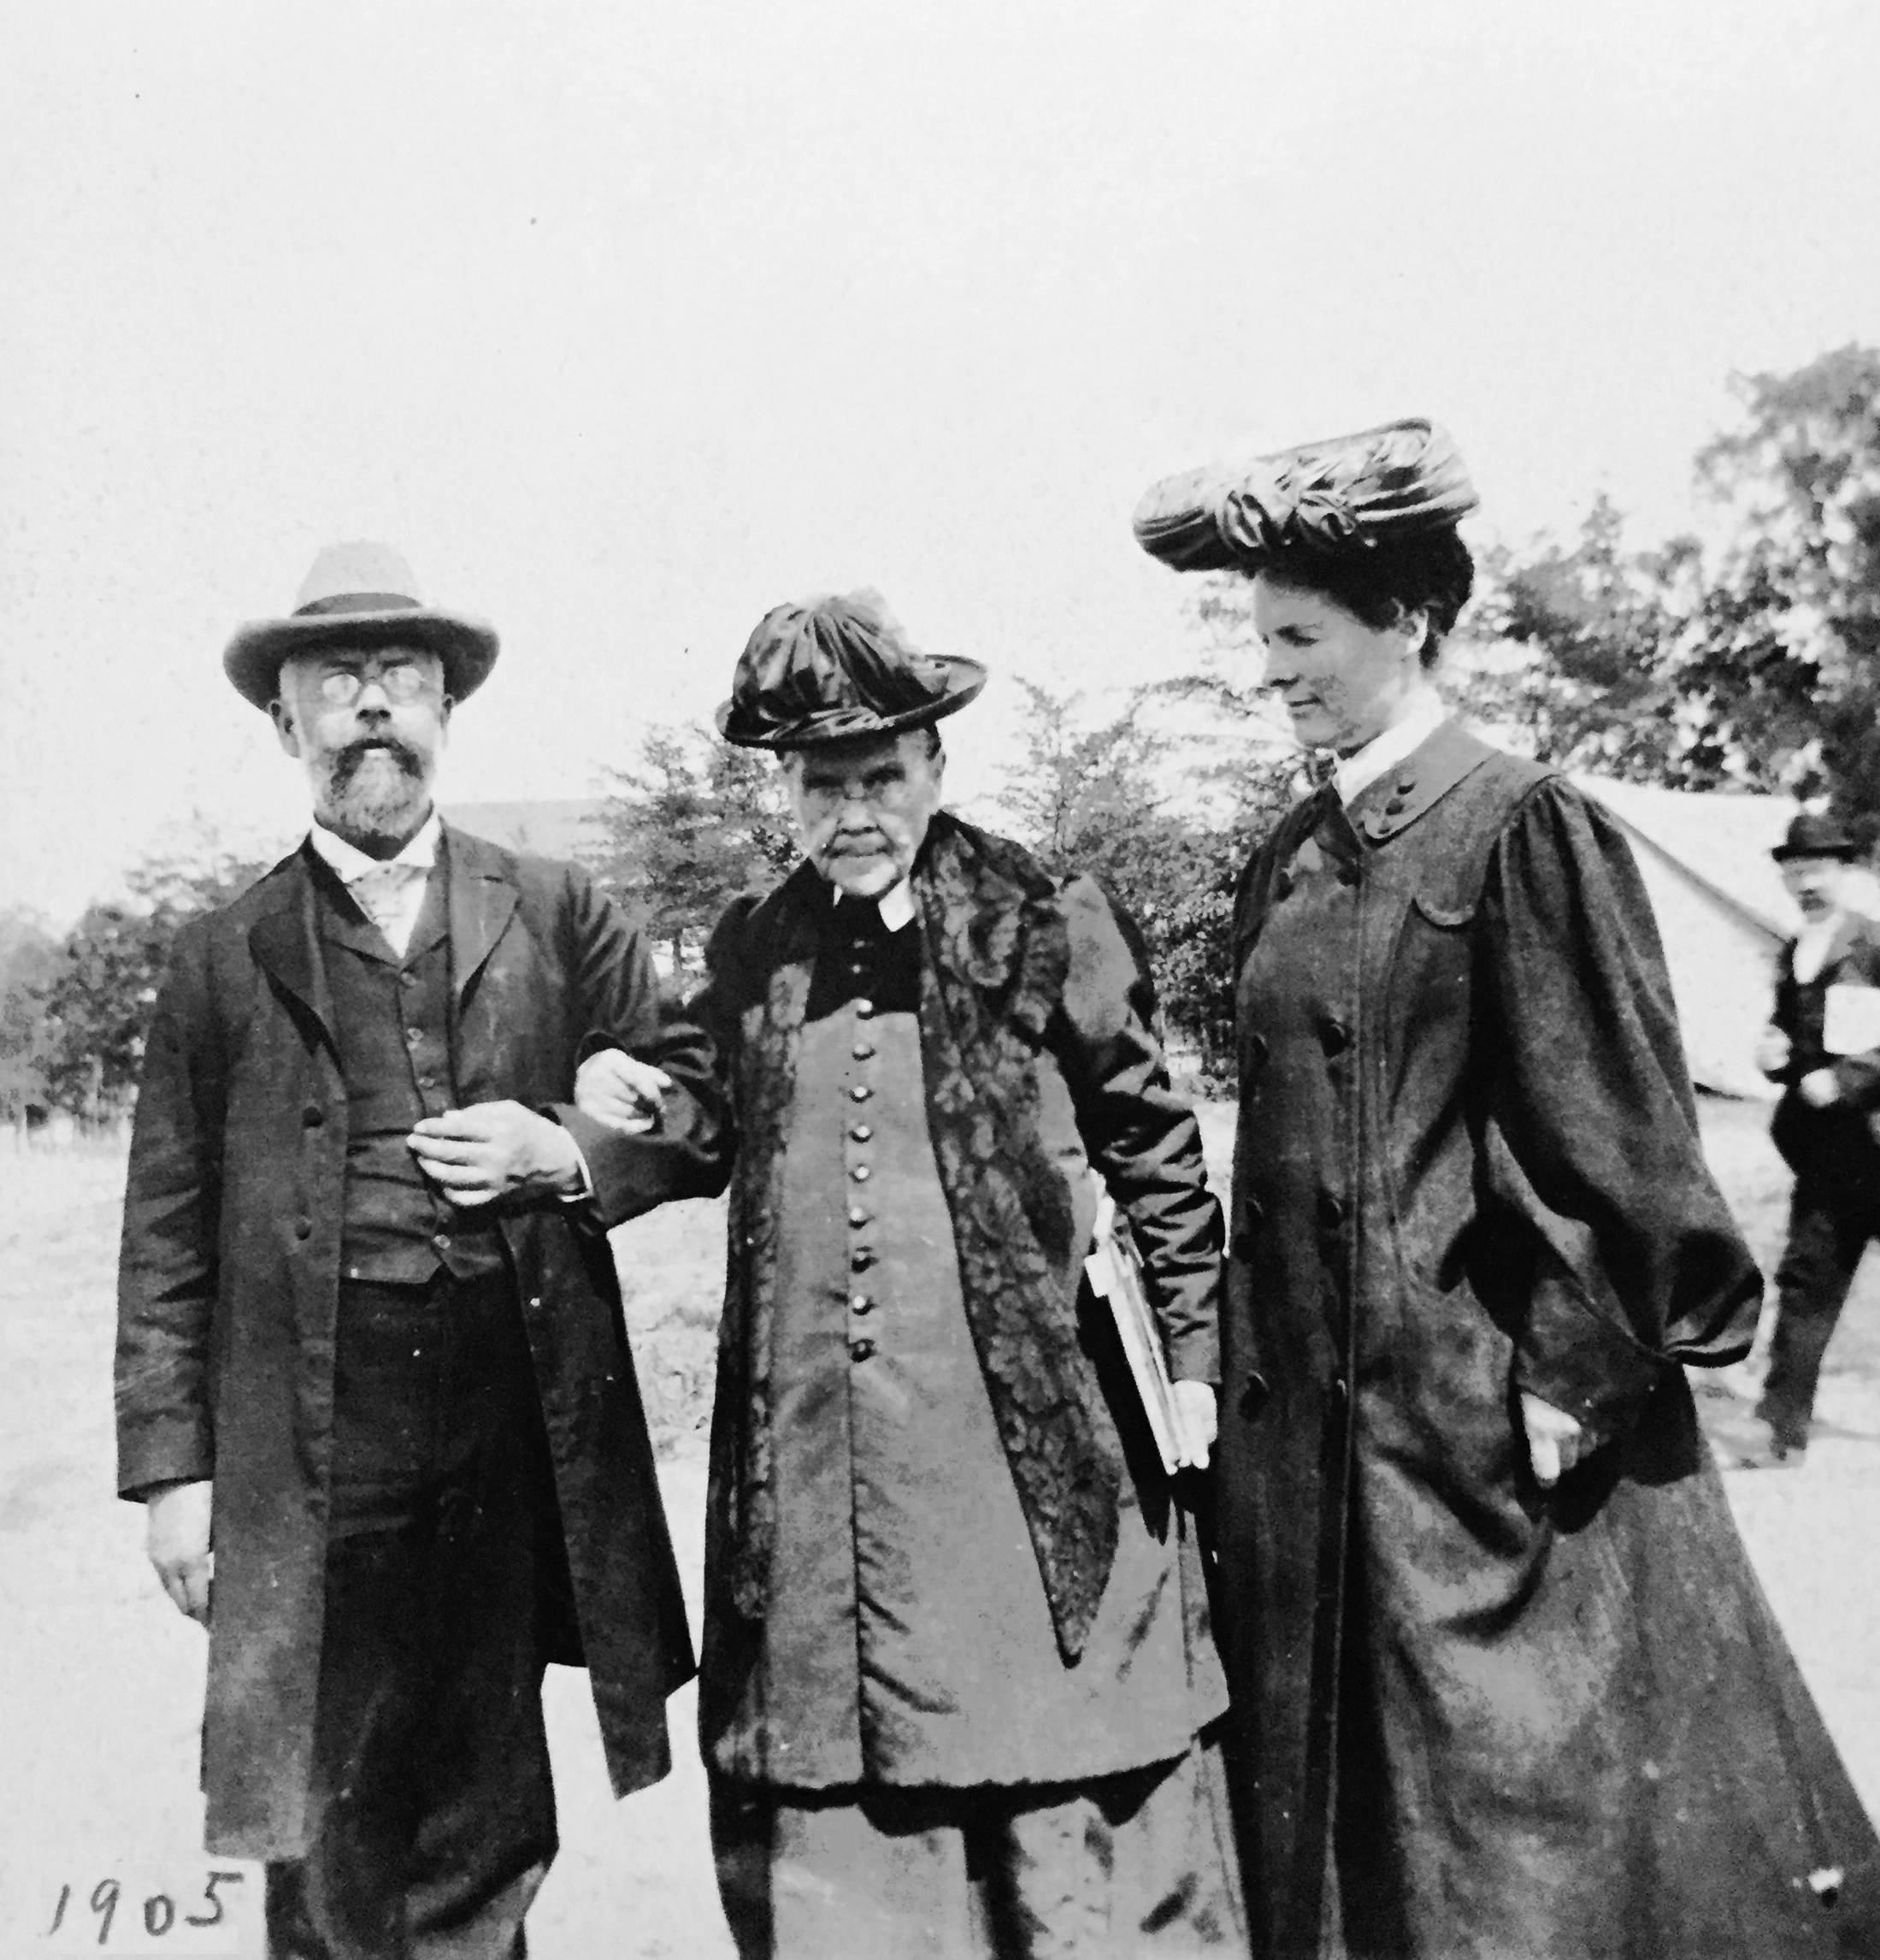
\includegraphics[width=1\linewidth]{images/william-ellen-white-1905.jpg}
    \caption*{William C. White i Ellen G. White, 1905}
    \label{fig:w-e-white}
\end{figure}

Według Williama White'a, naszą jedyną nadzieją jako Adwentystów Dnia Siódmego jest trzymanie się pierwotnych zasad. Te zasady, jak wiemy, to \emcap{Fundamentalne Zasady}. Następnie odniósł się do kolejności, w jakiej wróg atakuje naszą pracę. Atak zaczyna się od naszego braku jedności, następnie dąży do osłabienia naszego szacunku dla szabatu i służby świątynnej, celuje w nasze zaufanie do Ducha Proroctwa, a w końcu skupia się na wprowadzeniu zamieszania w nasze pojmowanie osobowego Boga.

Odpowiedź siostry White do Williama White'a ma zaskakujący charakter. Sugeruje nam, że wielkie odstępstwo wkrótce się urzeczywistni, a naszą nadzieją jest trzymanie się pierwotnych zasad naszej wiary — \emcap{Fundamentalnych Zasad}.

\egwnodot{Elmshaven, St. Helena, Kalifornia} \\
\egwnodot{4 grudnia 1905 r.} \\
\egwnodot{W. C. White} \\
\egwnodot{Mój drogi synu,}

\egw{\normaltext{[...]}}

\egw{\textbf{Jedno jest pewne, że wkrótce nadejdzie \underline{wielkie odstępstwo}, które rozwija się, zwiększa i rośnie w siłę, i \underline{będzie postępować}, aż Pan zstąpi z nieba z okrzykiem. \underline{Musimy trzymać się pierwotnych zasad naszej denominacyjnej wiary} i iść naprzód od tego, co mocne, do zwiększonej wiary. \underline{Zawsze} musimy zachowywać wiarę, która została potwierdzona przez Świętego Ducha Bożego \underline{od wcześniejszych wydarzeń naszego doświadczenia aż do obecnego czasu}.} Potrzebujemy teraz szerszej perspektywy i głębszej, bardziej żarliwej, niezachwianej wiary w prowadzenie Ducha Świętego. \textbf{Skoro potrzebowaliśmy wyraźnego dowodu mocy Ducha Świętego, aby potwierdzić prawdę \underline{na początku}, po upływie czasu, to \underline{potrzebujemy wszystkich dowodów na potwierdzenie prawdy dzisiaj}, gdy dusze odchodzą od wiary i dają posłuch zwodniczym duchom i naukom demonów}. Nie może być teraz żadnego osłabienia duszy. Jeśli kiedykolwiek był czas, kiedy potrzebowaliśmy mocy Ducha Świętego w naszych przemówieniach, w naszych modlitwach, w każdym proponowanym działaniu, to jest on teraz. \textbf{Nie możemy zatrzymać się na pierwszym doświadczeniu, ale gdy głosimy ludziom \underline{to samo poselstwo}, \underline{poselstwo to ma być wzmocnione i poszerzone}}. \textbf{Musimy dostrzec i zrozumieć znaczenie poselstwa, które stało się pewne dzięki swemu boskiemu pochodzeniu}. Musimy dążyć do poznania Pana, abyśmy wiedzieli, że Jego wyjście jest przygotowane jak poranek. Nasze dusze potrzebują ożywienia ze Źródła wszelkiej mocy. \textbf{{Możemy być wzmocnieni i utwierdzeni w doświadczeniu z przeszłości, \underline{trzymającym nas przy istotnych punktach prawdy, które uczyniły nas tym, czym jesteśmy — Adwentystami Dnia Siódmego}}}}[Lt326-1905.2; 1905][https://egwwritings.org/read?panels=p7678.8]

\egwnogap{\textbf{Ostatnie pięćdziesiąt lat nie przyćmiło ani jednej joty czy zasady naszej wiary, tak jak ją przyjęliśmy, wraz z wielkimi i cudownymi dowodami, które zostały nam dane jako pewne w roku 1844, po upływie czasu.} Słabnące dusze mają być wzmocnione i ożywione zgodnie z Jego Słowem. I wielu kaznodziejów ewangelii oraz lekarzy Pana będzie miało swoje osłabione dusze ożywione zgodnie ze Słowem. \textbf{\underline{Ani jedno słowo nie zostało zmienione ani zanegowane}.} \textbf{To, co Duch Święty poświadczył jako prawdę po upływie czasu, w naszym wielkim rozczarowaniu, jest \underline{solidnym fundamentem prawdy}. Filary prawdy zostały objawione i przyjęliśmy \underline{fundamentalne zasady}, które uczyniły nas tym, czym jesteśmy — Adwentystami Dnia Siódmego, przestrzegającymi przykazań Bożych i mającymi wiarę Jezusa}}[Lt326-1905.3; 1905][https://egwwritings.org/read?panels=p7678.9]

Ten list jest zaskakujący, ponieważ jest odpowiedzią na sposób, w jaki wróg atakuje nasze dzieło. Siostra White jest w pełni świadoma tych ataków i przedstawiła problem we właściwym świetle, pokazując nam również, co powinniśmy zrobić, aby zapobiec atakom szatana na nas. Wróg chce \othersnodot{wprowadzić zamieszanie nasze pojmowanie osobowego Boga}. To jest właśnie sedno wielkiego odstępstwa, które \egwinline{wkrótce nadejdzie}, i które \egwinline{rozwija się, zwiększa i rośnie w siłę, i będzie postępować, aż Pan zstąpi z nieba z okrzykiem}. To jest odstępstwo, którego doświadczamy dzisiaj. Jaka jest nasza nadzieja przeciwko temu zwiedzeniu i wielkiemu odstępstwu? \egwinline{\textbf{\underline{Mamy mocno trzymać się pierwotnych zasad naszej denominacyjnej wiary} i iść naprzód od tego, co mocne, do zwiększonej wiary. \underline{Zawsze} musimy zachowywać wiarę, która została potwierdzona przez Świętego Ducha Bożego od wcześniejszych wydarzeń naszego doświadczenia aż do obecnego czasu}}.
\egwinline{\normaltext{[...]} \textbf{\underline{poselstwo to  ma być wzmocnione i poszerzone}} \normaltext{[...]}} \egwinline{\normaltext{[...]} \textbf{\underline{potrzebujemy wszystkich dowodów na potwierdzenie prawdy dzisiaj}} \normaltext{[...]}} \egwinline{\textbf{Możemy być wzmocnieni i utwierdzeni w doświadczeniu z przeszłości, trzymającym nas przy istotnych punktach prawdy, które uczyniły nas tym, czym jesteśmy — Adwentystami Dnia Siódmego}}. Te istotne punkty prawdy, które uczyniły nas Adwentystami Dnia Siódmego, to \emcap{Fundamentalne Zasady}, zrodzone na początku naszej pracy. W 1905 roku napisała, \egwinline{\textbf{Ostatnie pięćdziesiąt lat nie przyćmiło ani jednej joty czy zasady naszej wiary, tak jak ją przyjęliśmy, wraz z wielkimi i cudownymi dowodami, które zostały nam dane jako pewne w roku 1844, po upływie czasu}}. \egwinline{\textbf{Ani jedno słowo nie zostało zmienione ani zanegowane.} \textbf{To, co Duch Święty poświadczył jako prawdę po upływie czasu, w naszym wielkim rozczarowaniu, jest \underline{solidnym fundamentem prawdy}. Filary prawdy zostały objawione i przyjęliśmy \underline{fundamentalne zasady}, które uczyniły nas tym, czym jesteśmy — Adwentystami Dnia Siódmego, przestrzegającymi przykazań Bożych i mającymi wiarę Jezusa}}.

Bóg wzywa nas do wytrwałości w \emcap{Fundamentalnych Zasadach}, szczególnie w kwestii \othersnodot{pojmowania osobowego Boga}. Jest to pierwszy punkt \emcap{Fundamentalnych Zasad}.

Siostra White przepowiedziała, że w naszym Kościele rozwija się wielkie odstępstwo dotyczące zrozumienia \emcap{osobowości Boga}. Prawdziwe zrozumienie \emcap{osobowości Boga} jest przedstawione w \emcap{Fundamentalnych Zasadach}. Wyraźnie ostrzegała nas przed atakiem szatana na te zasady. Wzywa nas, aby mocno \egw{\textbf{trzymać się pierwotnych zasad naszej denominacyjnej wiary} i iść naprzód od tego, co mocne, do zwiększonej wiary}

\egw{\textbf{Po upływie czasu, Bóg powierzył swoim wiernym naśladowcom cenne \underline{zasady teraźniejszej prawdy}. Te zasady nie zostały dane tym, którzy nie mieli udziału w głoszeniu poselstwa pierwszego i drugiego anioła. Zostały one dane pracownikom, którzy mieli udział w tym dziele od początku}}[Ms129-1905.5; 1905][https://egwwritings.org/read?panels=p9797.12]

\egwnogap{\textbf{Ci, którzy przeszli przez te doświadczenia, mają być \underline{mocni jak skała wobec zasad}, które uczyniły nas Adwentystami Dnia Siódmego}. Mają być współpracownikami Boga, wiążąc świadectwo i pieczętując prawo wśród Jego uczniów. Ci, którzy brali udział w ustanawianiu naszej pracy na fundamencie biblijnej prawdy; \textbf{ci, którzy znają drogowskazy, które wskazały właściwą ścieżkę}, mają być uznani za pracowników najwyższej wartości. Mogą mówić z osobistego doświadczenia o powierzonych im prawdach. Ci ludzie nie powinni pozwolić, aby ich wiara zmieniła się w niewiarę; nie powinni pozwolić, aby sztandar trzeciego anioła został zabrany z ich rąk. Mają trzymać się swoich początkowych wierzeń mocno aż do końca. \textbf{\underline{Pan oświadczył, że historia z przeszłości powtórzy się, gdy będziemy wkraczać w końcowe dzieło}. Każda prawda, którą dał na te ostatnie dni, ma być ogłoszona światu. \underline{Każdy filar}, który ustanowił, \underline{ma być wzmocniony}. Nie możemy teraz zejść z fundamentu, który Bóg ustanowił. Nie możemy teraz wejść w żadną nową organizację; oznaczałoby to odstępstwo od prawdy}}[Ms129-1905.6; 1905][https://egwwritings.org/read?panels=p9797.13]

Odejście od fundamentu, który Bóg ustanowił, oznacza wejście w nową organizację; to jest odstępstwo od prawdy. Gdy porówna się \emcap{Fundamentalne Zasady} z przeszłości z obecnymi trynitarnymi Fundamentalnymi Wierzeniami, widać wyraźnie, że znajdujemy się w stanie odstępstwa. Ellen White przepowiedziała, że to odstępstwo będzie \egwinline{\textbf{rozwijać się, zwiększać i rosnąć w siłę, i \underline{będzie postępować}, aż Pan zstąpi z nieba z okrzykiem}}[Lt326-1905.2; 1905][https://egwwritings.org/read?panels=p7678.8].

\begin{titledpoem}

    \stanza{
        To kryzys w liście przewidziany, \\
        Przez Ellen White zapowiedziany. \\
        „Wróć do korzeni!”, bo będzie źle, \\
        Więc odstępstwa tego strzeżcie się.
    }

    \stanza{
        Fundament prawdy z wczesnych dni \\
        Jest pod atakiem — prorok drży. \\
        „Przeciwstaw się!” — to jej zadanie, \\
        Bo się nasz okręt nie ostanie.
    }

    \stanza{
        „Złapcie się zasad!” — krzyk dochodzi, \\
        Czasu proroczego dowodzi. \\
        Prawda przez Ducha objawiona \\
        Nie będzie nigdy znieważona.
    }

    \stanza{
        Swym sprytem szatan buja statkiem, \\
        By nagle kurs zmienić ukradkiem. \\
        Lecz takich zachwiań się nie boi \\
        To serce, co na prawdzie stoi.
    }

    \stanza{
        Oprzyjmy się na tym, co znamy, \\
        Na tych Zasadach, które mamy, \\
        W których zawarta życia droga \\
        Pod okiem tak świętego Boga.
    }

    \stanza{
        I chociaż świat szybko przemija, \\
        Prawda się z Ellen ust przebija. \\
        Światłem latarni nas prowadzi \\
        I wiernym w ich podróży radzi.
    }

\end{titledpoem}

